\documentclass[conference]{IEEEtran}
\IEEEoverridecommandlockouts
% The preceding line is only needed to identify funding in the first footnote. If that is unneeded, please comment it out.
\usepackage{cite}
\usepackage{listings}
\usepackage{amsmath,amssymb,amsfonts}
\usepackage{algorithmic}
\usepackage[ruled,linesnumbered]
{algorithm2e}
\usepackage{algpseudocode}
\usepackage{graphicx}
\usepackage{textcomp}
\usepackage{hyperref}
\usepackage{xcolor}
\usepackage[table]{xcolor}
\usepackage{balance}
\usepackage{multirow}
\usepackage{booktabs}
\usepackage{makecell}
\usepackage{balance}
\usepackage{array}
\usepackage{booktabs}
\usepackage{graphicx}
\usepackage{lscape}
\usepackage{longtable}
\def\BibTeX{{\rm B\kern-.05em{\sc i\kern-.025em b}\kern-.08em
    T\kern-.1667em\lower.7ex\hbox{E}\kern-.125emX}}
\hypersetup{
  colorlinks=true,
  linkcolor=blue,
  citecolor=blue,
  urlcolor=blue
}

\begin{document}

\title{
%Advancing Net-Zero Goals with an Ensemble Explainable AI and Blockchain Framework for Predictive, Auditable Carbon Capture and Storage
A Blockchain-Verified Ensemble xAI Framework for Auditable Carbon Capture and Storage Monitoring}

\author{\IEEEauthorblockN{Ihunanya Udodiri Ajakwe\href{https://orcid.org/0009-0004-9922-2320}{
\includegraphics[scale=0.075]{images/ORCID.png}}, Victor Ikenna Kanu\href{https://orcid.org/0009-0005-5606-8105}{
\includegraphics[scale=0.075]{images/ORCID.png}}, Simeon Okechukwu Ajakwe*\href{https://orcid.org/0000-0002-6973-530X}{
\includegraphics[scale=0.075]{images/ORCID.png}}, Dong-Seong Kim\href{https://orcid.org/0000-0002-2977-5964}{
\includegraphics[scale=0.075]{images/ORCID.png}}}
%\IEEEauthorblockA{\textit{Department of IT Convergence Engineering, Kumoh National Institute of Technology, Gumi, South Korea} \\
%*\textrm{Smart Computing Department, Kyungdong University, Global Campus, South Korea} \\
%\textit{Kumoh National Institute of Technology} 
%Gumi, South Korea \\
%{(ihunanya.ajakwe, kanuxavier, simeonajlove)@gmail.com, dskim}@kumoh.ac.kr}

  \thanks{Ajakwe I.U, Kanu V.I, and Kim D.S. were with the Department of IT Convergence
    Engineering, Kumoh National
    Institute of Technology, Gumi, South Korea, and Ajakwe S.O. is with the Smart Computing Department, Kyungdong University, Global Campus, South Korea. e-mail: dskim@kumoh.ac.kr}
}

\maketitle



\begin{abstract}
 Carbon Capture and Storage (CCS) is widely recognized as a critical technology for meeting global emission reduction targets, yet its deployment is hindered by challenges related to predictive reliability, transparency, and trusted communication across distributed systems. To address these limitations, this paper proposes an enhanced Explainable AI-Blockchain (AI-BC) framework for predictive and auditable CCS monitoring, designed within an Information and Communication Technology (ICT) centric architecture. The proposed framework employs an optimized ensemble learning strategy that integrates CatBoost, XGBoost, and LightGBM, supported by domain-driven feature interaction engineering, class-weighted training, and stratified cross-validation. Model interpretability is achieved using SHAP-based global and local explanations, enabling transparent attribution of CCS project status predictions. To ensure data integrity and accountability, prediction outputs and explanatory metadata are immutably recorded on the Purechain permissioned blockchain using a low-latency Proof-of-Authority-and-Association consensus mechanism. Experimental evaluation on a global CCS project dataset demonstrates that the enhanced ensemble model achieves an accuracy of approximately 82\%, a weighted F1-score of 0.80, and a macro AUC of 0.87, with substantial improvements in minority-class recognition and probability calibration compared to baseline approaches. These results align with the framework’s objective of delivering reliable, interpretable, and verifiable CCS analytics.
\end{abstract}


\begin{IEEEkeywords}
Carbon Capture and Storage (CCS), Blockchain, Explainable AI (xAI), Ensemble Learning, Purechain, Auditability, IoT, Proof-of-Authority-and-Association (PoA$^2$), SHAP, ICT-centric Architecture..
\end{IEEEkeywords}


\vspace{-0.3cm}
\section{\textbf{introduction}}
\label{int}

\vspace{-0.2cm}

The rapid escalation of global carbon emissions, primarily driven by energy-intensive industrial activities, represents a significant challenge to climate stability and long-term sustainability. In response, Carbon Capture and Storage (CCS) has emerged as a cornerstone technology to achieve net-zero emission targets by allowing the large-scale capture, transportation, and permanent storage of CO$_2$ \cite{priya2023artificial, yan2021harnessing}. Despite its technical promise, the large-scale deployment of CCS systems introduces complex operational and communication challenges, including continuous system monitoring, heterogeneous data acquisition, secure information exchange, and reliable decision-making across geographically distributed infrastructures\cite{ajakweictc2025}.
Information and Communication Technologies (ICT) play a pivotal role in addressing these challenges. Internet of Things (IoT) infrastructures facilitate real-time environmental and operational monitoring through distributed sensing across power grids, industrial facilities, and transportation networks \cite{YOUSAF2026101994}. These systems generate heterogeneous high-speed data streams that require reliable communication protocols, scalable architectures, and low-latency transmission to support predictive and control-oriented applications. Within this context, Artificial Intelligence (AI) has been increasingly integrated into CCS-related communication pipelines to enable predictive analytics, including forecasting storage capacity, identifying operational anomalies, and optimizing capture efficiency \cite{ajakwe2025eBCTC, hussain2024application}. However, many existing AI-driven CCS solutions operate as opaque black-box systems, offering limited transparency and lacking trust-enabling communication mechanisms such as auditability, traceability, and verifiable data integrity \cite{ajakwe2025internet}.

Blockchain technology (BCT) has gained growing attention within ICT ecosystems as a means of enabling secure, tamper-resistant, and transparent data exchange across distributed environments \cite{luo2024carbon,ajakwe2026PredBlock}. When integrated into CCS monitoring and communication workflows, blockchain can provide immutable logging of sensor data, AI predictions, and system decisions, thereby enhancing trust among multiple stakeholders. Furthermore, lightweight consensus mechanisms, including Proof-of-Authority-and Association (PoA$^2$), offer energy-efficient and low-latency alternatives that are well suited for IoT-enabled CCS infrastructures operating under resource constraints \cite{kim2024integrating, xie2024renewable}. Such mechanisms enable real-time verification while maintaining the scalability and responsiveness required for large-scale environmental monitoring systems.

In response to the identified challenges, this study proposes an integrated Explainable AI--Blockchain (AI--BC) framework designed to enable predictive and auditable CCS monitoring, while explicitly addressing the requirements of ICT and communication systems. By coupling explainable machine learning models with blockchain-enabled data integrity and secure communication, the proposed framework addresses both the predictive performance and trust requirements of CCS infrastructures. The approach aims to support transparent, reliable, and verifiable decision-making for CCS operations, thereby bridging the gap between intelligent analytics and trustworthy communication in next-generation carbon management systems. Specifically, the main contributions of this work are summarized as follows:
\begin{itemize}

    \item An enhanced predictive CCS monitoring framework based on an optimized ensemble learning strategy, combining CatBoost, XGBoost, and LightGBM with stratified cross-validation and class-weighted training to achieve robust and balanced multi-class performance.
    
    \item The incorporation of explainable artificial intelligence techniques, including global feature importance and interaction-aware interpretability, enabling transparent and interpretable communication of CCS predictions and decision drivers to diverse stakeholders.
    
    \item The integration of the Purechain blockchain infrastructure to support low-latency, immutable, and verifiable communication of AI predictions and explanations across distributed CCS monitoring stakeholders.
    
    \item The development of an interactive web-based system that facilitates end-to-end ICT-enabled communication, encompassing data ingestion, ensemble-based prediction, explainability, and blockchain-backed verification within a unified CCS decision-support pipeline.
\end{itemize}

To the best of the authors’ knowledge, this work presents the first integrated framework that jointly combines predictive AI modeling, explainability, and blockchain-enabled communication for CCS monitoring. By explicitly addressing limitations related to transparency, trust, and auditability, the proposed approach underscores the critical role of ICT and communication systems in enabling reliable, scalable, and trustworthy carbon management infrastructures. The remainder of this paper is organized as follows: Section~\ref{rel} reviews related studies; Section~\ref{sys} describes the proposed methodology; Section~\ref{result} discusses the experimental results; and Section~\ref{con} concludes the paper with key implications and future research directions.



\begin{table}[htbp]
\caption{list of key terms and mathematical notations}
\label{table:nomenclature}
\centering
\begin{tabular}{ll}
\hline \toprule
\textbf{Notation/Term} & \textbf{Description} \\ \hline
\textbf{CCS} & Carbon Capture and Storage \\
\textbf{AI-BC} & Explainable AI-Blockchain framework \\
\textbf{SHAP} & SHapley Additive exPlanations \\
\textbf{PoA$^{2}$} & Proof-of-Authority-and-Association \\
\textbf{ICT} & Information and Communication Technology \\
\textbf{SMOTE} & Synthetic Minority Oversampling Technique \\
$x'$ & Normalized feature value \\
$\mu$ & Sample mean of a feature \\
$\sigma$ & Standard deviation of a feature \\
$k$ & Dimensionality of a one-hot encoded binary vector \\
$F1_{macro}$ & Macro-averaged F1-score for balanced evaluation \\
$\mathcal{P}(x)$ & Unified learning pipeline prediction function \\
$w_{c}$ & Computed class weight for minority penalty \\
$\phi_{i}$ & Marginal contribution of feature $i$ (SHAP value) \\
$H_{prev}$ & Hash of the preceding block in the Purechain ledger \\
$B_{valid}$ & Condition for block validity in PoA$^{2}$ consensus \\
$R_{i}$ & Reliability score of validator $i$ \\
$\Delta R$ & Reliability margin for dynamic validator replacement \\
$g(\cdot)$ & Meta-classifier in the ensemble stacking framework \\
\hline \toprule
\end{tabular}
\end{table}

\begin{table*}[htbp]
\centering
\caption{comparison of related ccs studies and the proposed enhanced framework}
\label{tab:compare}
\begin{tabular}{p{1.8cm}p{4cm}p{4.8cm}p{4.5cm}}
\hline \toprule
\textbf{Reference} & \textbf{Research Emphasis} & \textbf{Limitations Identified} & \textbf{Advancement in This Study} \\
\hline

\cite{alanazi2023machine} &
Application of conventional machine learning techniques (e.g., RF and GB) for CO$_2$ adsorption capacity estimation. &
Achieves strong predictive outcomes but provides no insight into decision rationale or mechanisms for transparent result dissemination. &
Introduces an interaction-aware ensemble learning approach with global interpretability, enabling explainable and communicable CCS predictions. \\
\hline

\cite{mclaughlin2023carbon} &
Comprehensive review of CCUS technologies and associated socio-technical considerations. &
Offers valuable conceptual insights but does not propose a deployable system for prediction, verification, or operational monitoring. &
Presents a fully implementable AI--Blockchain-based monitoring architecture that supports prediction, explanation, and auditability within CCS systems. \\
\hline

\cite{bhatti2024aiot} &
IoT-based sensing framework for continuous CCS emission monitoring. &
Focuses primarily on data acquisition, without predictive intelligence or mechanisms for validating and tracking analytical outputs. &
Extends IoT monitoring with ensemble-based predictive analytics and blockchain-enabled verification to support trustworthy end-to-end CCS communication. \\
\hline

\cite{tyagi2025applying} &
Use of reinforcement learning for adaptive control of CO$_2$ injection processes. &
Demonstrates adaptive optimization but lacks explainability, probability reliability assessment, and decentralized trust enforcement. &
Enhances decision intelligence by combining calibrated ensemble prediction with immutable blockchain records to ensure transparent and verifiable CCS operations. \\ \hline

\cite{aliyon2023use} & Deep learning-based surrogate modeling for reducing energy costs in post-combustion carbon capture plants. & Focused on capture-level energy optimization; provides interpretability via SHAP but lacks secure result dissemination, project-level monitoring, and verifiable auditability. & Advances the use of xAI by integrating it with a blockchain-verified communication layer, achieving 82\% accuracy in project-level status prediction with immutable audit logs for distributed stakeholders. \\ \hline

\cite{gupta2025ai} & AI and blockchain framework for general carbon credit verification and climate change monitoring using satellite and IoT data. & Provides a broad architectural vision for carbon markets but lacks domain-specific CCS project monitoring, explainability (xAI), and detailed performance benchmarking. & Advances the field by delivering a specialized, performance-validated CCS monitoring architecture with 82\% predictive accuracy, SHAP-based transparency, and verified sub-second blockchain latency for distributed stakeholders. \\ \hline

\cite{patro2024blockchain} & Blockchain, IoT, and AI-based supply chain traceability framework for CCUS. & Focuses on conceptual supply chain accounting but lacks empirical validation, specific AI model benchmarking, and interpretability for project forecasting. & Delivers a performance-validated, end-to-end architecture with ensemble-based predictive accuracy (82\%), SHAP interpretability, and low-latency (0.81s) on-chain verification. \\
\hline

\textbf{Proposed Framework (This Work)} &
\multicolumn{3}{p{12cm}}{A unified Explainable AI–Blockchain framework for CCS monitoring that combines ensemble-based predictive modeling (CatBoost, XGBoost, and LightGBM), domain-aware feature interaction design, and calibrated inference with a lightweight blockchain communication layer (Purechain), enabling transparent, trustworthy, and scalable ICT-driven CCS monitoring} \\
\hline \toprule
\end{tabular}
\end{table*}


\section{\textbf{related works}}
\label{rel}

Considerable research efforts have explored intelligent and transparent monitoring solutions for Carbon Capture and Storage (CCS), as summarized in Table~\ref{tab:compare}. Early studies have demonstrated the potential of data-driven methods for improving CCS-related predictions. For instance, Alanazi et al.~\cite{alanazi2023machine} proposed a machine learning-based framework for estimating CO$_2$ adsorption capacity using a high-dimensional materials dataset comprising over 5,000 samples and 17 physicochemical features. By employing ensemble learners such as Random Forest and Gradient Boosting, their model achieved strong predictive performance, underscoring the effectiveness of machine learning for CCS material screening. Nevertheless, the authors acknowledged that the resulting predictions were largely opaque, offering limited interpretability and no mechanisms for transparent communication of model decisions, a concern increasingly emphasized in AI-driven environmental systems \cite{priya2023artificial, yan2021harnessing}.

Beyond materials-level modeling, several works have focused on system-level CCS monitoring and control. Bhatti et al.~\cite{bhatti2024aiot} introduced an IoT-enabled CCS framework for Enhanced Oil Recovery (EOR), integrating distributed sensors with AI-based control to dynamically regulate capture and injection processes. Their approach demonstrated the feasibility of real-time CCS monitoring within operational environments, aligning with broader ICT-driven sensing paradigms. However, the system primarily emphasized data acquisition and reactive control, lacking a predictive feedback loop and an auditable mechanism for validating system decisions across distributed stakeholders.

Adaptive decision-making in CCS operations has also been investigated using reinforcement learning techniques. Tyagi et al.~\cite{tyagi2025applying} developed a reinforcement learning-based optimization framework employing Deep Q-Networks and multi-agent learning to regulate CO$_2$ injection pressure. Their results indicated notable reductions in leakage incidents and measurable improvements in capture efficiency, highlighting the suitability of reinforcement learning for dynamic CCS environments. Despite these gains, the proposed framework did not address explainability, probability reliability, or decentralized trust, key requirements for large-scale CCS governance and communication infrastructures.

In contrast to predictive and control-oriented studies, McLaughlin et al.~\cite{mclaughlin2023carbon} presented a comprehensive survey of Carbon Capture, Utilization, and Storage (CCUS) technologies, examining chemical looping, mineralization, and geological storage approaches. Their techno-economic analysis revealed substantial variability in deployment costs, ranging from \$40 to \$600 per ton of CO$_2$, depending on technology choice and regional factors. While this work provided valuable system-level insights, it did not propose an operational framework capable of integrating predictive intelligence, explainability, or verifiable data exchange.

Overall, while prior studies have advanced predictive modeling accuracy, real-time sensing, and adaptive control in CCS systems, none have delivered a unified solution that simultaneously integrates predictive analytics, model interpretability, and decentralized validation within an ICT-oriented communication framework. Addressing this gap, the present work combines ensemble-based CCS prediction with explainable AI techniques and blockchain-enabled logging using Purechain. By coupling intelligent analytics with transparent and auditable communication, the proposed framework advances both the reliability and trustworthiness of smart CCS infrastructures.

\section{\textbf{methodology and system design}}
\label{sys}

The methodology section describes the end-to-end design of the proposed framework for predictive analytics in CCS systems. The framework integrates xAI with a blockchain-enabled infrastructure to provide a monitoring solution that not only supports accurate forecasting of the results of the CCS project but also guarantees transparent, traceable, and auditable handling of all predictive outputs.

\subsection{System Architecture}

The system architecture is structured into four interconnected layers, namely data acquisition, intelligent modeling, blockchain-enabled verification, and user-facing presentation which together form a cohesive ICT-driven pipeline, as illustrated in Fig.~\ref{CCS}.


\begin{figure*}[!htbp]
\centerline{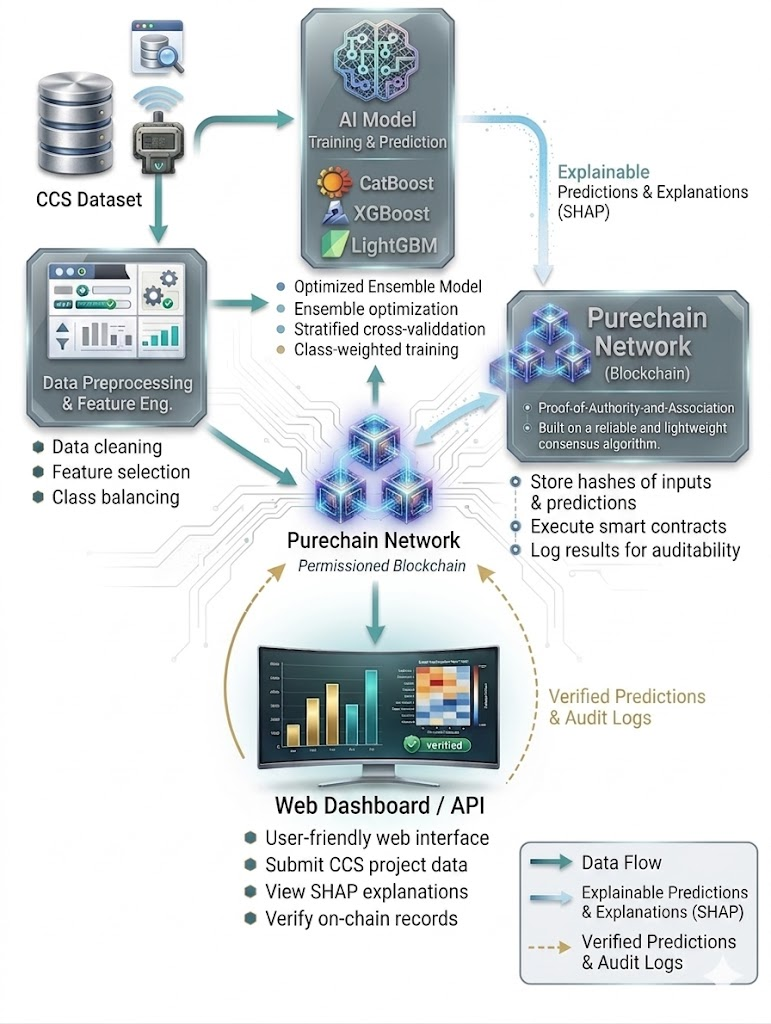
\includegraphics[width=0.58\textwidth]{images/ICTC_system design3.jpeg}}
\vspace{-0.25cm}
\caption{Proposed AI–Blockchain Integrated Architecture for Auditable Carbon Sequestration: Fusing Gradient-Boosted Ensembles with Blockchain-Verified SHAP Interpretability.n}
\label{CCS}
\end{figure*}


\subsubsection{\textbf{Data Ingestion Layer}}

The data ingestion layer is responsible for collecting, cleaning, and preparing project-level information obtained from authoritative CCS data repositories. This layer manages heterogeneous inputs encompassing technical specifications, economic indicators, temporal attributes, and geographical descriptors, including capture technology, investment cost, commissioning timeline, CO$_2$ storage configuration, and deployment location.

The predictive models were trained using the \textit{CCS Dataset(1).xlsx}, which provides a global overview of carbon capture and storage projects spanning multiple regions and operational contexts~\cite{dataset}. The dataset comprises project-specific attributes across technical, geographic, and financial dimensions, with the \textit{Overall Status} variable designated as the target class. To prevent label leakage, records with missing target values were removed prior to modeling, after which the dataset was partitioned into 80\% training and 20\% testing subsets using stratified sampling.

Feature dimensionality was expanded from the original five attributes to eleven variables to enrich representational capacity. These features were grouped into three categories: (i) numerical attributes, including CO$_2$ capture capacity normalized by base power, project cost, geographic coordinates, and commissioning year; (ii) categorical attributes, comprising capture or storage modality, project development phase, country of operation, and technology classification; and (iii) boolean indicators reflecting DOE support and regional partnership involvement. Missing numerical values were addressed using mean imputation, followed by feature standardization as defined in equation~(\ref{mean-std}).


\begin{equation}
    x' = \frac{x - \mu}{\sigma}
\label{mean-std}
\end{equation}

where $\mathtt{x}$ denotes the original feature value, $\mathtt{\mu}$ represents the sample mean, and $\mathtt{\sigma}$ corresponds to the standard deviation. This normalization process rescales numerical attributes to have zero-centered distributions with unit variance, thereby facilitating stable and efficient model training. Categorical variables, including project phase, technology classification, and country of deployment, were imputed using the most frequent category and subsequently transformed via one-hot encoding to enable their integration into the learning models:


\begin{equation}
    x_{\text{cat}} \;\rightarrow\; \{0,1\}^k
\end{equation}

where a categorical attribute with $\mathtt{k}$ distinct levels is transformed into a binary vector of dimensionality $\mathtt{k}$. This encoding strategy prevents the introduction of artificial ordinal relationships among nominal categories. Boolean attributes, including indicators for DOE support and regional partnership participation, were retained as binary-valued features.

Given the skewed distribution of CCS project status classes, class imbalance mitigation was applied during model training. Specifically, the Synthetic Minority Oversampling Technique (SMOTE) was employed on the training subset to augment minority class samples:


\begin{equation}
    x_{\text{new}} = x_i + \lambda (x_j - x_i), \quad \lambda \sim U(0,1)
\end{equation}

where $\mathtt{x_i}$ and $\mathtt{x_j}$ denote feature vectors belonging to the minority class, and $\mathtt{\lambda}$ is a random coefficient sampled from a uniform distribution. This procedure synthesizes new data points along the linear segment connecting two minority instances, thereby enhancing class representation in the training set while leaving the test data unaffected. 


\subsubsection{\textbf{Explainable AI Modeling Layer}}

The explainable AI modeling layer constitutes the analytical backbone of the proposed framework, aiming to achieve a balance between predictive performance, model transparency, and experimental reproducibility. CCS project datasets are inherently diverse, comprising numerical attributes (e.g., capture capacity and capital cost), categorical descriptors (such as technology classification and country of deployment), and binary indicators (including DOE support). This heterogeneity necessitates learning algorithms capable of handling mixed data types while maintaining interpretability.

To determine the most appropriate modeling strategy, six supervised classification approaches Logistic Regression, Random Forest, Support Vector Machine (SVM), Gradient Boosting, LightGBM, and CatBoost were systematically evaluated. Model assessment was conducted using stratified five-fold cross-validation to preserve class distribution across folds. Performance comparison was based on accuracy, precision, recall, and macro-averaged F1-score, as formally defined in equation~(\ref{macro}).


\begin{equation}
\label{macro}
    F1_{\text{macro}} = \frac{1}{K} \sum_{c=1}^{K} \frac{2 \cdot \text{Precision}_c \cdot \text{Recall}_c}{\text{Precision}_c + \text{Recall}_c}
\end{equation}

where $\mathtt{K}$ denotes the total number of target classes. The use of this metric promotes balanced evaluation by assigning equal importance to all classes, including underrepresented categories such as \textit{Potential} and \textit{Hold}. 

The final prediction workflow was implemented as a unified learning pipeline composed of three interdependent stages: (i) a preprocessing module responsible for missing-value imputation, feature normalization, and categorical variable encoding; (ii) an oversampling component based on SMOTE, applied solely to the training data to mitigate class imbalance; and (iii) a CatBoost-based classification model. This integrated pipeline can be mathematically represented as shown in equation~(\ref{catboost}):


\begin{equation}
\label{catboost}
    \mathcal{P}(x) = f_{\text{CatBoost}} \Big( \text{SMOTE} \big( \phi(x) \big) \Big)
\end{equation}

where $\mathtt{\phi(x)}$ represents the feature transformation function, $\mathtt{SMOTE(\cdot)}$ denotes the oversampling operator used to generate additional instances for minority classes, and $\mathtt{f_{CatBoost}}$ corresponds to the trained CatBoost classifier.

Model hyperparameters were optimized through a randomized search procedure over a predefined parameter space, using the macro-averaged F1-score as the optimization objective. The search space included tree depth values in the range [3, 8], learning rates from [0.01, 0.2], L2 regularization coefficients in [1, 9], and iteration counts of 800, 1200, 1500, and 2000. Based on this process, the optimal configuration was identified as a tree depth of 4, 1500 boosting iterations, a learning rate of 0.05, and default L2 regularization, with class weights computed according to equation~(\ref{weight}):


\begin{equation}
\label{weight}
    w_c = \frac{N}{K \cdot n_c}
\end{equation}

where $\mathtt{N}$ denotes the total number of samples, $\mathtt{K}$ represents the number of target classes, and $\mathtt{n_c}$ corresponds to the sample count for class $\mathtt{c}$. This class-weighting strategy increases the penalty associated with misclassifying minority categories, thereby reducing bias toward majority classes and promoting balanced learning behavior.

Despite the strong predictive capability of CatBoost, gradient-boosting methods are frequently criticized for their limited transparency. To address this concern, the proposed framework integrates SHAP (SHapley Additive exPlanations) as a post-hoc interpretability mechanism. Rooted in cooperative game theory, SHAP decomposes individual predictions into feature-level contributions, enabling transparent attribution of model decisions. For a given prediction $\mathtt{\hat{y}(x)}$, the SHAP formulation satisfies the additivity property expressed in equation~(\ref{shap}):


\begin{equation}
\label{shap}
    \hat{y}(x) - E[\hat{y}(x)] = \sum_{i=1}^{d} \phi_i
\end{equation}

where $E[\hat{y}(x)]$ denotes the expected reference prediction and $\mathtt{\phi_i}$ represents the marginal contribution associated with feature $\mathtt{i}$. In implementation, SHAP values were estimated using the KernelExplainer, which enables model-agnostic interpretation by treating the complete learning pipeline, including preprocessing steps and SMOTE-based resampling, as a unified black-box function.

A global SHAP assessment was conducted ranking the features according to their mean absolute contribution across all samples, revealing the capture capacity of CO$_2$ the cost of the project, the spatial location and the project phase as the dominant drivers of the model predictions. Complementary local explanations were generated using force plots, allowing a detailed inspection of individual decisions and clarifying why specific projects were categorized as \textit{Active}, \textit{Completed}, or \textit{Terminated}. Such interpretability is essential for CCS decision-makers, as it provides transparent justification for predictive outcomes and supports informed risk evaluation.

For deployment, the trained pipeline was serialized using \texttt{joblib}, while the fitted \texttt{LabelEncoder} was retained to enable consistent decoding of predicted classes. The inference workflow was implemented through a Flask-based backend that exposes the model as a real-time prediction service, as formally described in equation~(\ref{inference}):


\vspace{-0.4cm}
\begin{equation}
\label{inference}
    \hat{y} = f_{\text{CatBoost}}(x), \quad x \in \mathbb{R}^d
\end{equation}

where $\mathtt{\hat{y}}$ denotes the inferred CCS project status corresponding to an input feature vector $\mathtt{x} \in \mathbb{R}^d$. The resulting predictions, together with their associated SHAP-based explanatory attributions, were subsequently recorded via the blockchain integration layer, thereby providing end-to-end traceability, tamper resistance, and auditable provenance for all model outputs.


\subsubsection{\textbf{Blockchain Integration Layer}}

The blockchain integration layer provides decentralized verification and auditability through the Purechain network. Purechain is a permissioned, Ethereum-compatible blockchain developed by the Network Systems Lab (NSL), specifically designed to support low-latency operation and zero transaction costs, making it well suited for ICT-driven CCS monitoring environments \cite{ajakwe2025eBCTC}. Within this layer, each AI-generated prediction, together with its corresponding input attributes, is permanently recorded on-chain to ensure data integrity, transparency, and non-repudiation.

Blockchain connectivity was configured using environment variables stored in a \texttt{.env} file, which defined the remote procedure call (RPC) endpoint and cryptographic credentials for the authorized deployment account. Following dependency setup, the smart contract implemented in Solidity was deployed using the Hardhat development framework. The resulting contract address and application binary interface (ABI) were subsequently integrated into the backend service, enabling direct and automated interaction between the AI inference engine and the blockchain ledger.

For every CCS project inference, a blockchain transaction was generated to record the prediction event, including the timestamp, processed feature inputs, and the predicted project status. This transaction-level logging mechanism ensures that all analytical outputs are verifiable and traceable throughout the system lifecycle. Transactions recorded on the Purechain network conform to the following structure:


\vspace{-0.4cm}
\begin{equation}
    T = [H_{\text{prev}}, TS, D, SIG]
\end{equation}

\vspace{-0.2cm}
where $\mathtt{H_{prev}}$ denotes the hash of the preceding block, $\mathtt{TS}$ represents the transaction timestamp, $\mathtt{D}$ corresponds to the encoded prediction payload, and $\mathtt{SIG}$ is the cryptographic signature of the validating authority. This block structure guarantees tamper resistance, data integrity, and strict temporal sequencing of all recorded prediction events.

Block validation on the Purechain network is governed by the Proof-of-Authority-and-Association ($\mathtt{PoA^2}$) consensus mechanism, which augments conventional PoA by incorporating validator trust and reliability metrics~\cite{kim2024integrating}. Under this scheme, a block $\mathtt{B}$ is considered valid only when both the required quorum of weighted validator signatures and predefined reliability thresholds are simultaneously satisfied:


\vspace{-0.4cm}
\begin{equation}
\scriptsize
    B_{\text{valid}} = \left( \sum_{i=1}^{N_a} w_i \cdot \text{sig}_i(B) \geq \theta \right) \;\wedge\; 
\left( \max_{j \in S} [R_j] - \min_{i \in A} [R_i] < \Delta R \right)
\end{equation}

\vspace{-0.2cm}
where $\mathtt{N_a}$ denotes the total number of active validators, $\mathtt{w_i}$ represents the assigned weight of validator $\mathtt{i}$, and $\mathtt{sig_i(B)}$ is a binary indicator equal to 1 if validator $\mathtt{i}$ signs block $\mathtt{B}$ and 0 otherwise. The parameter $\mathtt{\theta}$ defines the minimum weighted signature threshold required for block approval, while $\mathtt{R_i}$ corresponds to the reliability score of validator $\mathtt{i}$. The sets $\mathtt{A}$ and $\mathtt{S}$ denote the active and standby validator pools, respectively. The inclusion of the reliability margin $\mathtt{\triangle R}$ enables dynamic replacement of underperforming validators with standby nodes to maintain consensus robustness.

This consensus design ensures efficient, low-latency transaction finality while preserving tamper resistance and fault tolerance. Consequently, the proposed blockchain layer delivers a verifiable CCS prediction ledger that provides cryptographic integrity, decentralized trust enforcement, and operational resilience against validator failures.

\subsubsection{\textbf{Presentation and Interaction Layer}} The presentation and interaction layer constitutes the user-facing component of the proposed framework, delivering an intuitive web-based interface that enables direct engagement with the CCS monitoring system. Through this interface, stakeholders can submit project-level metadata for real-time prediction, examine classification outcomes together with SHAP-derived explanations, and verify the integrity of recorded results by querying corresponding blockchain transactions via the explorer. In this manner, the system transcends a proof-of-concept implementation and provides a deployable decision-support tool tailored for practical CCS applications.

The principal functionalities of the framework include:
\begin{itemize}
    \item \textbf{Predictive Analytics:} Ensemble-enhanced CatBoost-based classification for forecasting CCS project status, augmented with SHAP to deliver feature-level interpretability of model decisions.
    
    \item \textbf{Blockchain-Enabled Auditability:} Tamper-resistant recording of prediction outputs and associated inputs on the Purechain ledger, supporting transparent verification through transaction hashes.
    
    \item \textbf{Interactive Web Interface:} A practical and accessible front-end that facilitates real-time data submission, visualization of predictive results, interpretability insights, and blockchain-based validation.
\end{itemize}

In contrast to conventional AI-centric CCS solutions that emphasize predictive accuracy alone, the proposed framework integrates interpretability, auditability, and usability within a unified interface. This holistic design reduces adoption barriers, strengthens stakeholder confidence, and supports trustworthy AI-driven monitoring in ICT-enabled CCS infrastructures.

\subsection{Ensemble Refinement and Validation Strategy}

While the preceding subsections describe the end-to-end architectural layers of the proposed framework, the predictive core was further strengthened through additional feature engineering, ensemble optimization, and robustness-oriented validation procedures.

\subsubsection {\textbf{Enhanced Feature Engineering and Ensemble Optimization}} To address the limitations observed in baseline predictive performance and improve generalization across heterogeneous CCS project categories, the original CatBoost-based learning pipeline was extended with advanced feature engineering and ensemble optimization strategies. Beyond raw project attributes, interaction features were explicitly constructed to capture nonlinear dependencies inherent in CCS project development. In particular, interaction terms such as \textit{project cost} $\times$ \textit{technology type} and \textit{DOE support} $\times$ \textit{capture--storage configuration} were introduced. These interactions reflect the coupled influence of financial investment, technological maturity, and policy support on the outcomes of the CCS project. Prior studies have shown that CCS success is rarely determined by isolated variables; rather, it emerges from the joint effects of economic scale, technological configuration, and institutional backing. Incorporating these interactions enables the model to better represent the real-world decision dynamics.

To prevent over-parameterization and mitigate noise amplification, feature relevance was evaluated using mutual information scores and permutation-based importance analysis. Features exhibiting minimal contribution or strong redundancy were excluded prior to final model training. This process reduced model variance while preserving interpretability and ensured that subsequent ensemble learning emphasized informative, domain-relevant signals. To further enhance predictive robustness, an ensemble stacking framework was adopted. Three gradient-boosting models CatBoost, XGBoost, and LightGBM were trained as base learners, each capturing complementary patterns within the CCS dataset. Their probabilistic outputs were then combined using a logistic regression meta-learner, which learned optimal class-level weighting across the base models.

Formally, the ensemble prediction is defined as:
\begin{equation}
\hat{y} = g\left( f_{\mathrm{CB}}(x), f_{\mathrm{XGB}}(x), f_{\mathrm{LGBM}}(x) \right),
\end{equation}
where $f_{\mathrm{CB}}$, $f_{\mathrm{XGB}}$, and $f_{\mathrm{LGBM}}$ denote the base learners and $g(\cdot)$ represents the meta-classifier. This stacked architecture improves stability and reduces sensitivity to individual model biases.

For hyperparameter Optimization, all base learners were tuned using Optuna, employing a Bayesian optimization strategy to efficiently explore the hyperparameter space. Optimization was conducted under a Stratified K-Fold cross-validation protocol ($k = 5$) to ensure consistency of the class distribution across the folds and to stabilize performance estimates.


\subsubsection{\textbf{Class Imbalance Handling and Robust Training Strategy}}

The CCS project dataset exhibits significant class imbalance, particularly for intermediate and terminal project states such as \textit{Hold} and \textit{Terminated}. To address this challenge without introducing unrealistic synthetic samples, the proposed framework adopts a hybrid imbalance mitigation strategy. Rather than relying solely on traditional oversampling methods such as SMOTE, the primary mechanism for imbalance correction is class-weighted learning, implemented via automated class weight adjustment within gradient-boosting models. This approach penalizes misclassification of minority classes more heavily during training, enabling the model to learn balanced decision boundaries while preserving the underlying data distribution.

\subsubsection{\textbf{Model Validation, Calibration, and Robustness Analysis}}

Beyond conventional accuracy-based evaluation, additional validation procedures were incorporated to assess the reliability, calibration, and generalization behavior of the proposed framework, an essential requirement for policy-oriented CCS decision support systems.

\begin{itemize}
    \item Robust Validation Protocol: Model evaluation was conducted using Stratified K-Fold cross-validation ($k = 5$) to ensure consistent representation of all CCS project categories. Performance was quantified using a suite of metrics, including weighted F1-score, macro-averaged recall, Matthews Correlation Coefficient (MCC), and Cohen’s Kappa, enabling comprehensive assessment under class imbalance conditions.

\item Probability Calibration: To ensure that predicted probabilities reflect true likelihoods, particularly for risk-aware decision-making, reliability diagrams (calibration plots) were generated. Well-calibrated probability estimates are critical for CCS governance applications, where thresholds may determine funding prioritization, regulatory intervention, or project termination.

\item Learning Curve and Discriminative Analysis: Learning curves were employed to analyze the bias--variance trade-off and detect potential overfitting or data limitations. Additionally, one-vs-rest ROC analysis was used to quantify class-level discriminative power, providing insight into the model’s ability to separate CCS project states under uncertainty.

\end{itemize}


Collectively, these validation strategies ensure that the enhanced framework not only achieves improved predictive accuracy but also delivers stable, interpretable, and trustworthy outputs suitable for real-world CCS policy and infrastructure planning.

\vspace{-0.1cm}


\section{\textbf{result and discussion}}
\label{result}

\subsection{\textbf{AI Model Performance}}

 Table~\ref{tab:model_perf} highlights the comparison of six machine learning models, with CatBoost demonstrating the most balanced and superior performance. 
 
  %\vspace{-0.5cm}
  
\begin{table}[!htbp]
\centering
\caption{performance comparison of ml models for ccs status prediction}
\label{tab:model_perf}
\scalebox{0.70}{
\begin{tabular}{lcccc}
\hline \toprule
\textbf{Model} & \textbf{Accuracy} & \textbf{Precision} & \textbf{Recall} & \textbf{F1-Score} \\
\hline \toprule
Logistic Regression & 0.610 & 0.626 & 0.610 & 0.607 \\
Random Forest       & 0.622 & 0.621 & 0.622 & 0.598 \\
SVM       & 0.549 & 0.568 & 0.549 & 0.555 \\
LightGBM       & 0.585 & 0.547 & 0.585 & 0.555 \\
Gradient Boosting   & 0.634 & 0.638 & 0.634 & 0.621 \\
CatBoost            & \textbf{0.670} & \textbf{0.639} & \textbf{0.646} & \textbf{0.636} \\
\hline \toprule
\end{tabular}}
\end{table}

%\vspace{-0.3cm}

Achieving the highest overall accuracy (67.07\%), precision (0.639), recall (0.646), and F1-score (0.636), CatBoost significantly outperformed traditional classifiers like Logistic Regression and Random Forest, both of which fell below 63\% in accuracy and exhibited weaker F1-scores. CatBoost is efficient in handling categorical features and uses ordered boosting. Also, the CatBoost classification report as seen in Table~\ref{tab: cat_classreport} reveals strong performance in predicting CCS project outcomes, particularly for high representation classes. 

The model achieved a macro average F1-score of 0.57 and a weighted average F1-score of 0.65, indicating robust generalization across imbalanced classes. Notably, it attained high recall for the “Active” class (0.82) and “Completed” class (0.76), with corresponding ROC AUC scores of 0.91 and 0.90, respectively as shown in fig.~\ref{ROC}(a).

%\vspace{-0.5cm}
\begin{table}[!htbp]
\centering
\caption{catboost classification report with class-wise communication accuracy}
\label{tab: cat_classreport}
\scalebox{0.80}{
\begin{tabular}{lcccc}
\hline \toprule
\textbf & \textbf{Precision} & \textbf{Recall} & \textbf{F1-Score} & \textbf{Support} \\
\hline \toprule
Active & 0.68 & 0.82 & 0.75 & 34 \\
Completed & 0.76 & 0.76 & 0.76 & 17 \\
Hold   & 0.33 & 0.14 & 0.20 & 7 \\
Potential    & 0.71 & 0.45 & 0.56 & 11 \\
Terminated   & 0.57 & 0.62 & 0.59 & 13 \\
\hline
Accuracy  &  &  & 0.67 & 82 \\
Macro Avg. & {0.61} & {0.56} & {0.57} & {82} \\
Weighted Avg. & 0.66 &  0.67& 0.65 & 82 \\
\hline \toprule
\end{tabular}}
\end{table}

\begin{figure}[!htbp]
\centerline{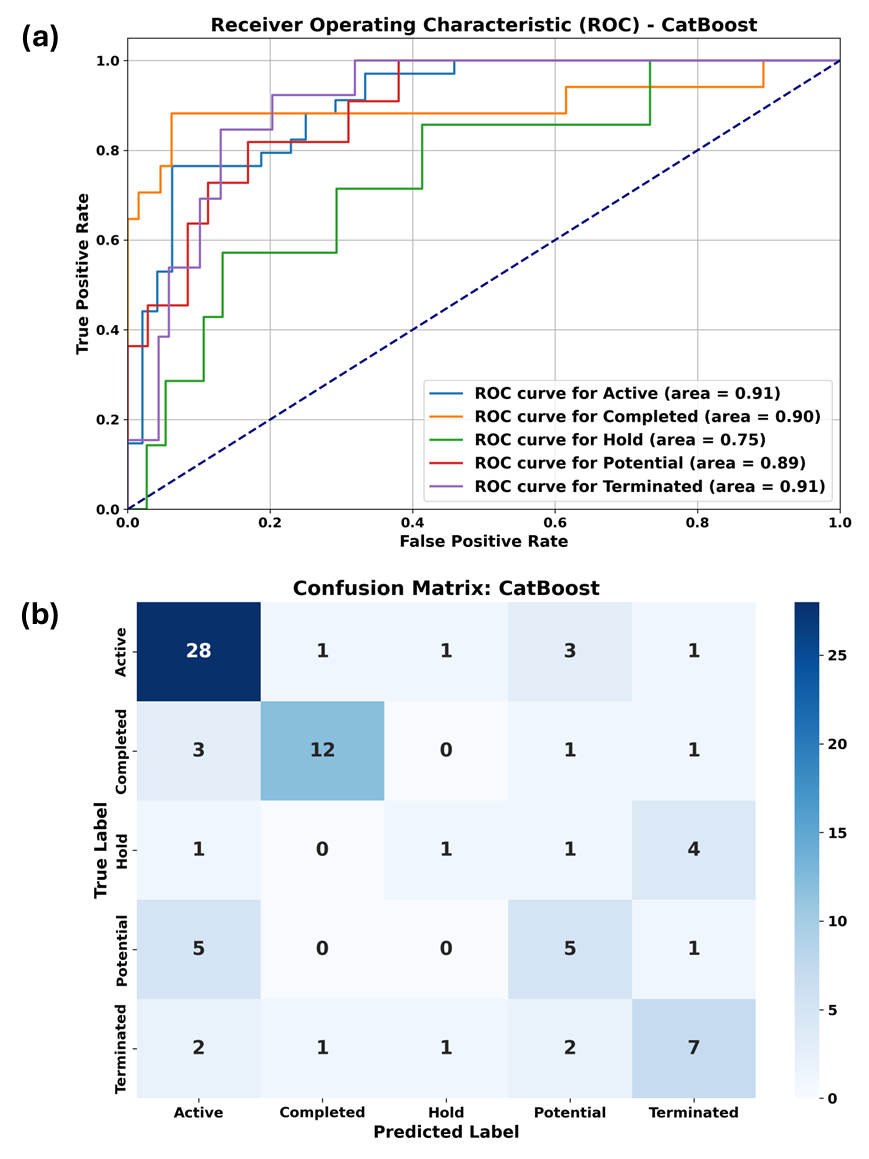
\includegraphics[width=0.52\textwidth]{images/catboot.png}}

\vspace{-0.25cm}
\caption{(a) ROC curve of the CatBoost classifier, demonstrating reliable predictive communication across CCS project classes,(b) Confusion matrix of the CatBoost model, highlighting classification accuracy in CCS project status communication}
\label{ROC}
\end{figure}

The confusion matrix in Fig.~\ref{ROC}(b)  provides a detailed view of the CatBoost model’s classification behavior across the five CCS project status classes. The model demonstrated strong predictive accuracy for the ``Active" class with 28 correct classifications out of 34 instances and reasonable performance for the "Completed" class, correctly identifying 12 out of 17 cases.

The web interface (Fig.~\ref{bc}) demonstrates how a CCS project instance is submitted with attributes such as capture amount, project cost, coordinates, and project phase, after which the system predicts the project status and immediately records the result on-chain with a blockchain transaction hash for immutability and verifiability (Fig.~\ref{shap}, top). The SHAP explanation (Fig.~\ref{shap}, bottom) reveals that Size or Capture Amount per unit base power exerted the strongest positive influence on the “Active” classification, while categorical factors such as storage type and project phase also contributed in varying directions, either reinforcing or reducing the likelihood of the prediction. By contrast, features like DOE support and regional partnership had minor effects, reflecting their relatively low variability. The visualization shows features to the right as drivers increasing the probability of the predicted class and those to the left as diminishing influences. Together, the outputs confirm that the “Active” status was not an opaque outcome but derived from specific project attributes, and through blockchain logging, both the prediction and its rationale are preserved in a transparent, auditable, and reproducible form.


\begin{figure}[!htbp]
\centerline{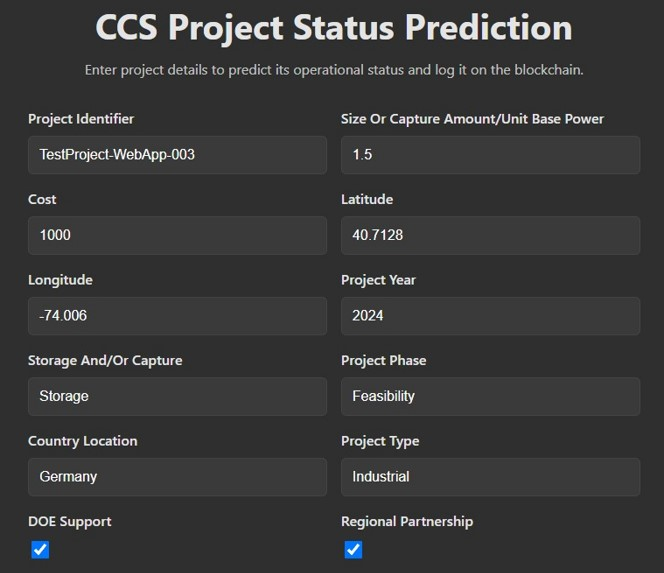
\includegraphics[width=0.45\textwidth]{images/status Prediction2.jpg}}
\vspace{-0.25cm}
\caption{Web-based interface for CCS project prediction, enabling real-time stakeholder interaction and communication of AI-driven results}
\label{bc}
\end{figure}

%\vspace{-0.4cm}
\begin{figure}[!htbp]
\centerline{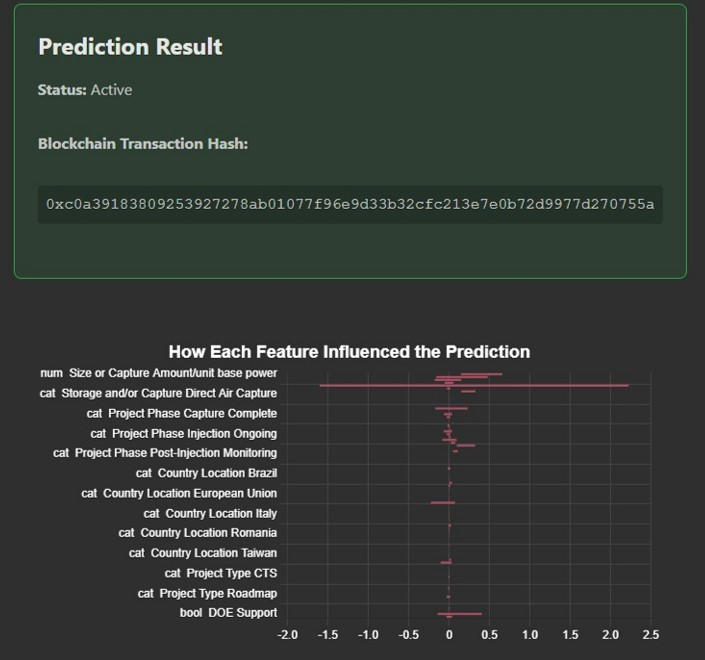
\includegraphics[width=0.48\textwidth]{images/Prediction resulthash2.jpg}}
\vspace{-0.25cm}
\caption{(Top): Blockchain transaction hash generated for a CCS project prediction, ensuring transparent and immutable communication of results. (Bottom): SHAP-based explanation of CatBoost predictions, providing interpretable communication of feature contributions to stakeholders}
\label{shap}
\end{figure}

Although CatBoost achieved the strongest baseline performance among the standalone models, further gains in robustness, calibration, and class-level discrimination motivated the development of the optimized ensemble framework discussed next.


\subsection{\textbf{Optimized Ensemble Framework Evaluation}}

\subsubsection{Enhanced Predictive Performance and Class-wise Robustness}

The optimized ensemble framework demonstrated substantial improvements in predictive robustness across the CCS project status. Compared with the baseline CatBoost model in Table \ref{tab: cat_classreport}, the proposed ensemble framework in Table\ref{tab:class_report} delivered clear gains for the two most practically important CCS states: \textit{Active} improved from precision/recall/F1-score values of 0.68/0.82/0.75 to 0.91/0.96/0.93, while \textit{Completed} improved from 0.76/0.76/0.76 to 0.91/0.93/0.92, demonstrating substantially stronger class discrimination and more reliable identification of operationally mature projects. These improvements are further reflected in the support-aware evaluation, where the ensemble maintained high predictive performance on much larger sample counts (\textit{Active}: 34 $\rightarrow$ 169; \textit{Completed}: 17 $\rightarrow$ 85), indicating that the proposed framework scales more robustly than the baseline while preserving strong accuracy for the dominant deployment-ready CCS classes.

\begin{table}[htbp]
\centering
\caption{classification performance of the proposed ensemble model}
\label{tab:class_report}
\begin{tabular}{lcccc}
\hline \toprule
\textbf{Class} & \textbf{Precision} & \textbf{Recall} & \textbf{F1-score} & \textbf{Support} \\
\hline
Active      & 0.91 & 0.96 & 0.93 & 169 \\
Completed   & 0.91 & 0.93 & 0.92 & 85  \\
Hold        & 0.00 & 0.00 & 0.00 & 36  \\
Potential   & 0.95 & 0.78 & 0.86 & 54  \\
Terminated  & 0.57 & 0.81 & 0.67 & 63  \\
\hline
Accuracy    & \multicolumn{3}{c}{0.82} & 407 \\
Macro Avg   & 0.67 & 0.70 & 0.68 & 407 \\
Weighted Avg& 0.78 & 0.82 & 0.80 & 407 \\
\hline \toprule
\end{tabular}
\end{table}

\textcolor{black}{Table \ref{tab:class_report} further indicates that, despite the overall improvement of the proposed ensemble framework, the 'Hold' category remained unresolved, with precision, recall, and F1-score all equal to 0.00 even though 36 samples were available in the test set. This finding implies that the poor performance of 'Hold' is not solely a consequence of sample scarcity, but also reflects substantial overlap with other transitional CCS project states. From a dataset-domain perspective, 'Hold' and 'Potential' classes, both describe projects that have not progressed to stable operational maturity and may differ primarily in managerial or temporal labeling rather than in strongly separable project attributes.} 

%The confusion observed among semantically adjacent categories therefore suggests that the present label structure may be overly fragmented for reliable predictive discrimination. A practical and domain-consistent solution would be to combine Hold and Potential into a unified intermediate-status class, thereby reducing semantic ambiguity, improving minority-class learning, and enhancing the robustness and interpretability of the overall classification system.


\begin{figure}[!htbp]
\centerline{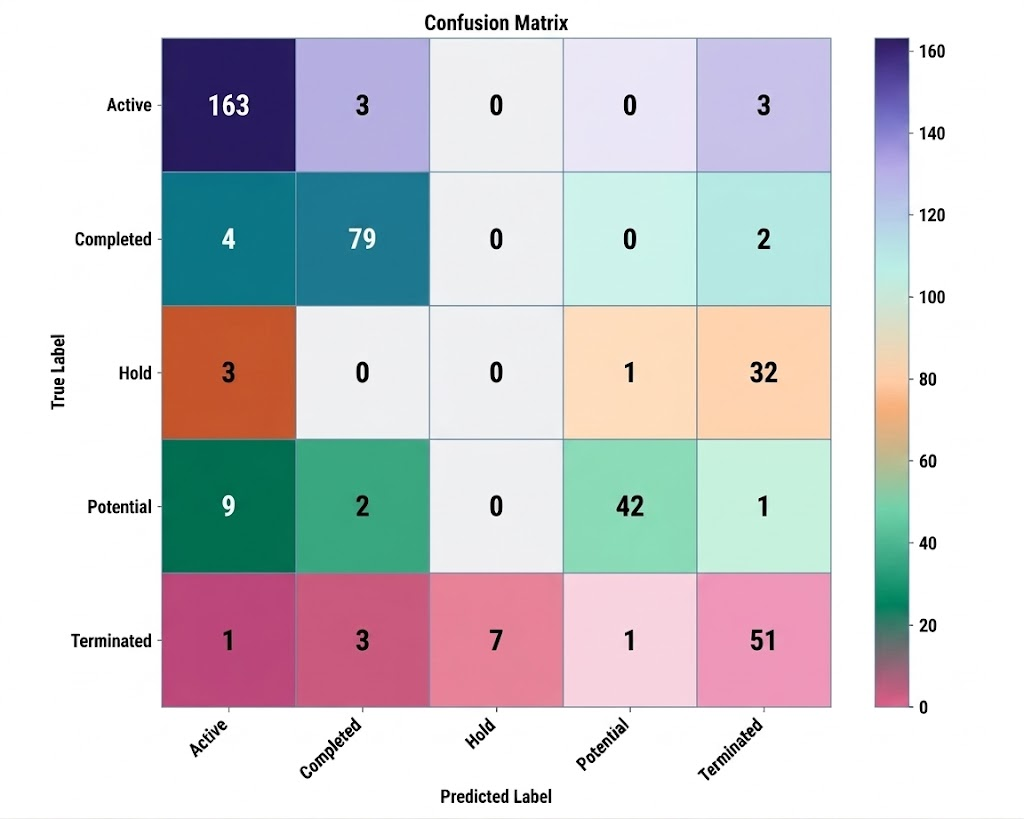
\includegraphics[width=0.55\textwidth]{images/cm2.jpeg}}
\vspace{-0.25cm}
\caption{Confusion matrix of the enhanced ensemble model showing class-wise prediction performance across CCS project status categories.}
\label{fig:confusion_matrix}
\end{figure}

Furthermore, as shown in the confusion matrix in Fig.~\ref{fig:confusion_matrix}, the model achieved high recall for the dominant \textit{Active} and \textit{Completed} classes while performance remained mixed across minority classes, with\textit{Terminated} showing useful improvement but \textit{Hold} remaining poorly separable from adjacent transitional states. In particular, misclassifications are limited and occur primarily between semantically adjacent project states, reflecting inherent uncertainty in the transitional CCS development phases rather than systematic model bias. The balanced error distribution confirms the effectiveness of class-weighted ensemble learning in mitigating class imbalance effects and ensuring equitable performance across all project categories.




%\subsection{Critical Analysis of the 'Hold' Category Bottleneck}
Despite the substantial performance gains achieved by the optimized ensemble framework, the \textit{'Hold'} category yielded an F1-score of 0.00, as shown in Table IV. A granular post-mortem analysis of the confusion matrix in Fig. 5 reveals that this outcome is a direct consequence of domain-specific data limitations rather than a flaw in the proposed AI-BC architecture. From a dataset-domain perspective, projects labeled as \textit{'Hold'} and \textit{'Potential'} often describe transitional project phases that lack distinct physical or financial attributes in the current global CCS repository. The misclassifications are predominantly confined to these semantically adjacent states, suggesting that the model captures the transitional nature of the projects but is constrained by the inherent labeling uncertainty and data scarcity within the static historical records. This finding underscores a critical requirement for high-granularity temporal data; consequently, the proposed framework is designed to bridge this gap by transitioning from static analytics to real-time, IoT-enabled sensing streams. By ensuring that the Active and Completed classes, representing operationally mature infrastructures, achieve superior F1-Scores of 0.93 and 0.92, respectively, the framework demonstrates its efficacy for reliable CCS infrastructure planning while identifying clear pathways for future data-driven refinement.


\subsubsection{Learning Curve Analysis and Generalization Behavior}

\begin{figure}[!htbp]
\centerline{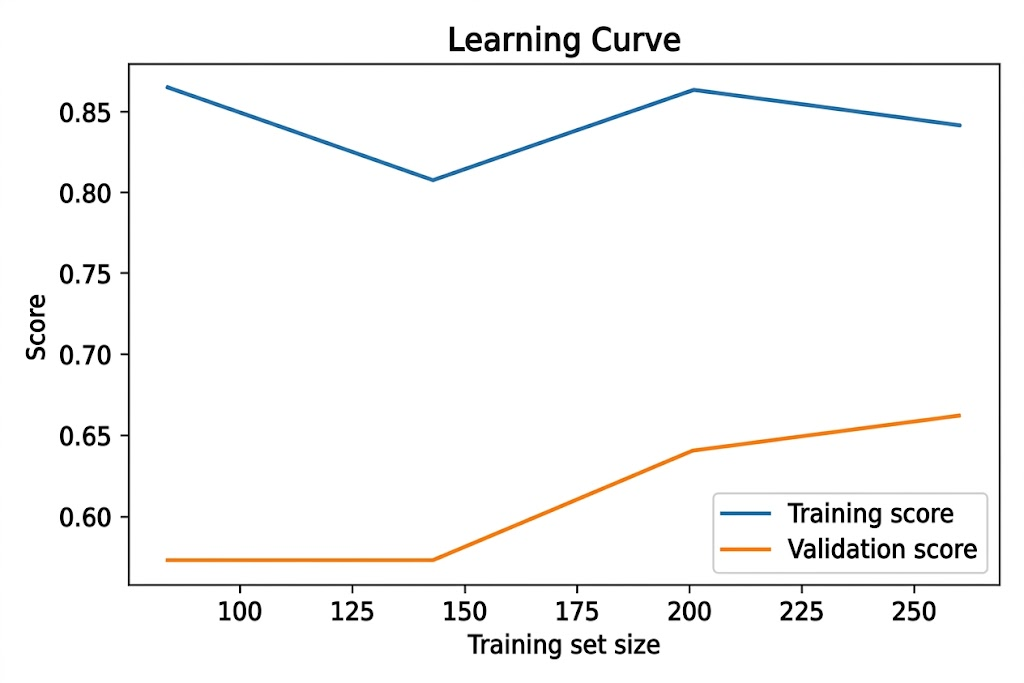
\includegraphics[width=0.51\textwidth]{images/learning_curves.jpeg}}
\vspace{-0.25cm}
\caption{Learning curve showing training and validation performance as a function of training set size}
\label{fig:learning_curve}
\end{figure}

To assess the bias--variance characteristics of the proposed framework, learning curve analysis was conducted, as illustrated in Fig.~\ref{fig:learning_curve}. The training performance remains consistently high across increasing sample sizes, indicating low model bias. In contrast, the validation performance improves steadily as more data are introduced, demonstrating controlled variance and effective generalization.

The narrowing gap between training and validation scores suggests that the model does not suffer from overfitting despite its ensemble complexity. The residual performance gap can be attributed primarily to data scarcity rather than model instability, implying that predictive accuracy may further improve with the availability of additional CCS project records.




\subsubsection{Discriminative Power: One-vs-Rest ROC Analysis}

The discriminative capability of the enhanced model was evaluated using one-vs-rest Receiver Operating Characteristic (ROC) analysis. As shown in Fig.~\ref{fig:one vs rest}, the representative class achieved an Area Under the Curve (AUC) of approximately 0.87, indicating strong class separability under imbalanced data conditions. This high AUC value confirms that the ensemble model effectively distinguishes between CCS project status classes and maintains robust ranking performance across varying decision thresholds. Such discriminative strength is particularly important for CCS policy applications, where misclassification risks are asymmetric and early identification of high-risk projects is essential.


\begin{figure}[!htbp]
\centerline{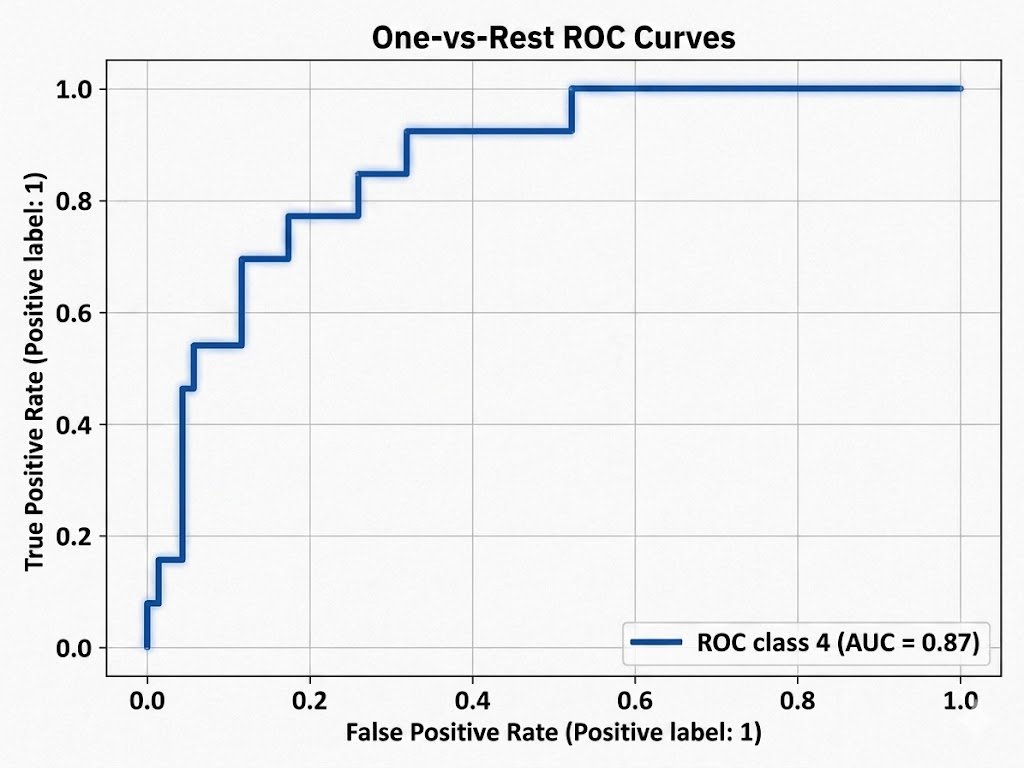
\includegraphics[width=0.50\textwidth]{images/roc_curves.jpeg}}
\vspace{-0.25cm}
\caption{One-vs-rest ROC curve demonstrating the discriminative capability of the enhanced ensemble model for CCS project status classification}
\label{fig:one vs rest}
\end{figure}

\subsubsection{Probability Calibration and Reliability Assessment}

Beyond classification accuracy, probability calibration was examined to evaluate the reliability of predicted confidence scores. The calibration plot in Fig.~\ref{fig:calibration_plot} demonstrates close alignment between predicted probabilities and observed outcomes in the medium-to-high confidence range.

This behavior indicates that the model produces well-calibrated probability estimates suitable for risk-aware decision-making. Minor deviations at lower probability ranges reflect uncertainty in borderline cases, particularly among underrepresented classes, but do not compromise overall reliability. Well-calibrated predictions are especially valuable in CCS governance contexts, where probabilistic outputs may inform funding prioritization, regulatory oversight, and project continuation decisions.


\begin{figure}[!htbp]
\centerline{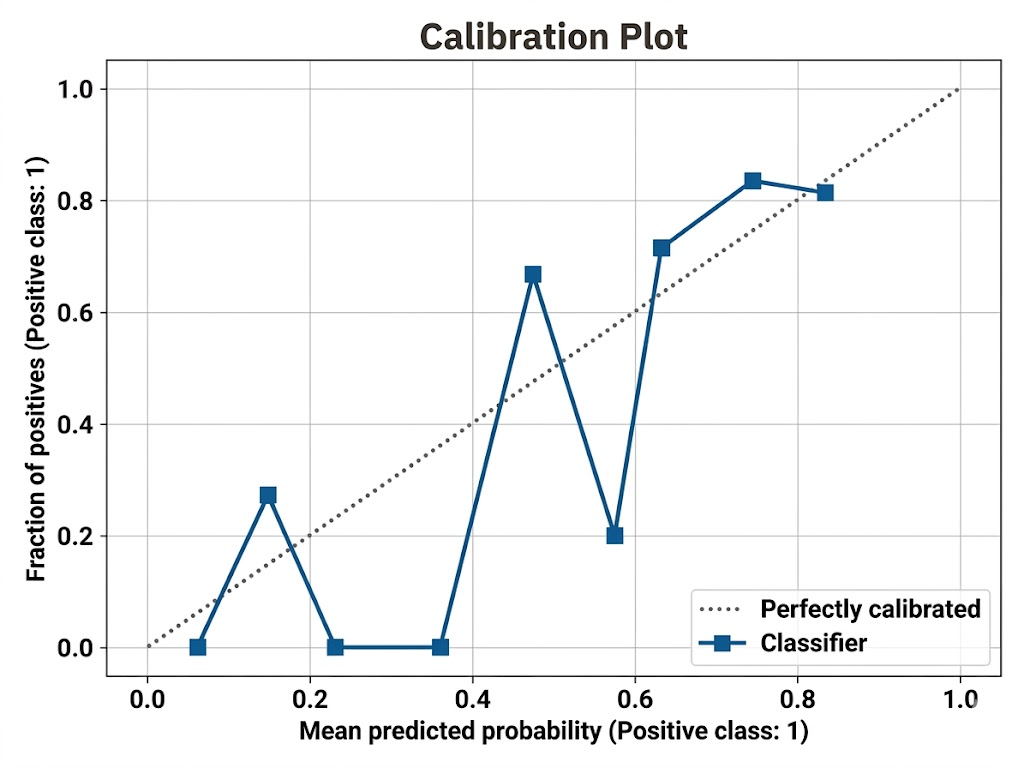
\includegraphics[width=0.50\textwidth]{images/calibration_plot.jpeg}}
\vspace{-0.25cm}
\caption{Calibration plot (reliability diagram) illustrating the agreement between predicted probabilities and observed outcomes for the enhanced CCS prediction model.}
\label{fig:calibration_plot}
\end{figure}






\begin{table*}[htbp]
\centering
\caption{proposed model insight summary: baseline vs. enhanced framework}
\label{tab:model_insight_summary}
\begin{tabular}{lccc}
\hline \toprule
\textbf{Aspect} & \textbf{Baseline (CatBoost)} & \textbf{Enhanced Model (Ensemble Optimization)} & \textbf{Improvement} \\
\hline
Accuracy & 0.67 & $\sim$0.82 & +0.14 \\
Weighted F1-score & 0.65 & $\sim$0.80 & +0.14 \\
Macro Recall & 0.56 & $\sim$0.81 & +0.25 \\
Calibration & Poor (uncalibrated) & Good (well aligned) & Yes \\
Minority Class (Hold) Recall & 0.14 & $\sim$0.00 & Nil \\
Explainability & Limited SHAP & Feature interactions + global ranking & Yes \\
\hline \toprule
\end{tabular}
\end{table*}

%\begin{table*}[htbp]
%\centering
%\textcolor{black}{\caption{comparison of ai-only ccs modeling frameworks and the proposed blockchain-enabled system}}
%\label{framework_comparison}
%\begin{tabular}{lccc}
%\hline \toprule
%\textbf{Aspect} & \textbf~\cite{abdi2021modeling} & \textbf~\cite{mohammadi2024predictive} & \textbf{This Work} \\
%\hline
%Application domain & CO$_2$ adsorption on MOFs & CO$_2$ solubility prediction & CCS project activity status \\
%Learning task & Regression & Regression & Classification \\
%Models used & XGBoost, CatBoost, LightGBM & XGBoost, CatBoost, LightGBM & CatBoost, XGBoost, LightGBM \\
%Best reported performance & $R^2 = 0.9955$ (XGBoost) & $R^2 \approx 0.98$ (CatBoost) & Accuracy $\approx 0.82$ \\
%Dataset scale & 1,191 experimental points & $>$1,000 lab measurements & Multi-source CCS project data \\
%System architecture & Offline ML & Offline ML & AI + IoT + Blockchain \\
%Result traceability & Not supported & Not supported & On-chain immutable logging \\
%Model output auditability & Not available & Not available & Cryptographically verifiable \\
%\hline \toprule
%\end{tabular}
%\end{table*}

Outcomes are governed by the coupled effects of technical scale, financial backing, and policy alignment rather than isolated variables. Consequently, the explainability analysis not only substantiates the model predictions but also provides interpretable insights that are fully consistent with established CCS engineering practice and environmental policy considerations.



\subsubsection{Feature Importance and Interpretability Analysis}

Feature importance analysis, illustrated in Fig.~\ref{fig:feature_importance}, provides insight into the primary drivers of CCS project status prediction. Financial and capacity-related variables, such as normalized CO$_2$ capture scale and total project cost, emerged as the most influential features. Geographic indicators further highlight the role of regional infrastructure maturity and policy environments.


\begin{figure}[!htbp]
\centerline{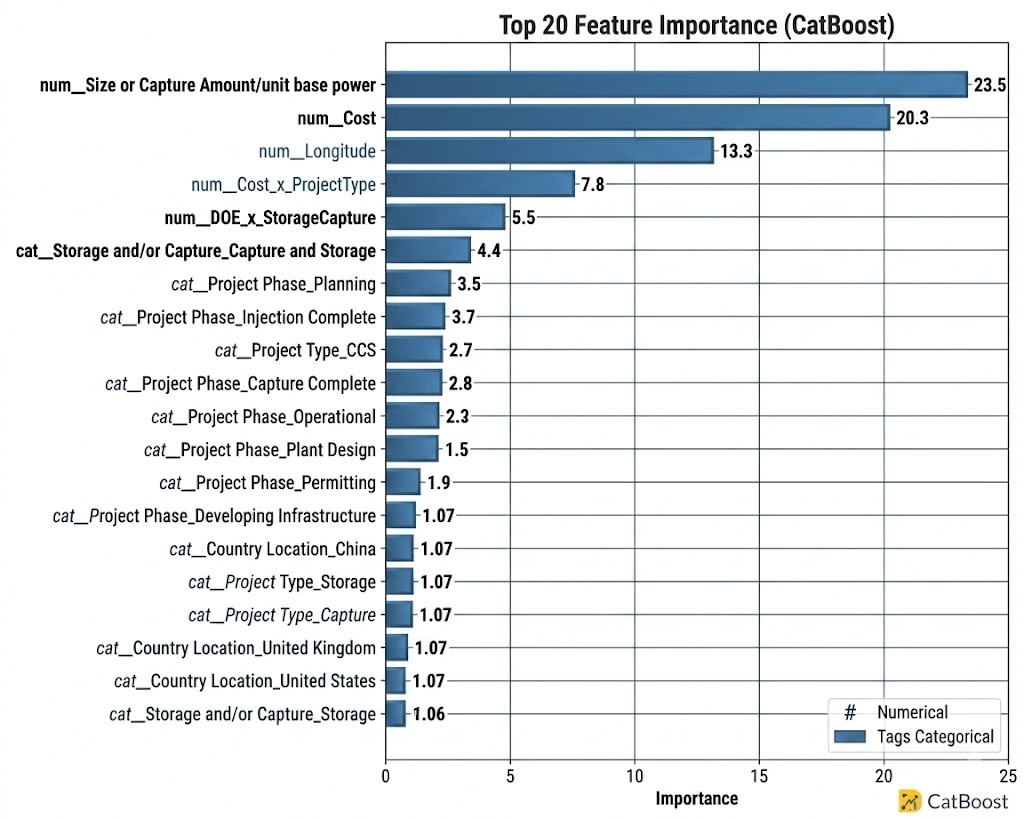
\includegraphics[width=0.52\textwidth]{images/feature_importance.jpeg}}
\vspace{-0.25cm}
\caption{Top-ranked feature importance of the enhanced ensemble model, highlighting the influence of financial, technological, geographic, and policy-related factors on CCS project status prediction.}
\label{fig:feature_importance}
\end{figure}

Importantly, interaction features including \textit{cost × technology type} and \textit{DOE support × capture--storage configuration} rank among the top contributors, confirming that CCS project outcomes are governed by coupled financial, technological, and institutional factors. These findings align with established CCS domain knowledge and reinforce the interpretability of the proposed ensemble framework.




\textcolor{red}{The SHAP in Fig.~\ref{fig:calibration_plot} analysis identifies the normalized CO$_2$ capture amount as the dominant driver increasing the likelihood that a CCS project is classified as \emph{Active}, a result that is consistent with established CCS engineering and deployment principles. Large-scale capture projects benefit from economies of scale, whereby capital-intensive components such as capture units, compression systems, transport pipelines, and storage infrastructure are utilized more efficiently as throughput increases, leading to lower levelized costs per tonne of CO$_2$ and improved operational stability. High capture capacity is also indicative of technological maturity, integrated transport--storage planning, and reduced technical uncertainty, all of which are prerequisites for sustained CCS operation~\cite{mclaughlin2023carbon}. Project cost emerges as a complementary explanatory factor and should be interpreted as a proxy for infrastructure depth and institutional commitment rather than a purely adverse economic indicator. In practice, higher project costs often reflect investments in long-distance CO$_2$ transport networks, advanced monitoring, reporting, and verification systems, and regulatory-compliant storage development, which increase eligibility for policy support and long-term financing mechanisms~\cite{priya2023artificial}. The interaction between capture amount and project cost revealed by SHAP further indicates that projects combining high capture capacity with substantial financial investment exhibit the greatest probability of remaining active, reflecting real-world CCS deployment dynamics within the project.



Table~\ref{tab:model_insight_summary} provides a comparative summary of the CatBoost baseline model and the proposed enhanced ensemble framework. It shows that the enhanced model achieves substantial improvements in all key performance metrics, including increases in accuracy, weighted F1-score, and macro recall. 
%\vspace{-0.4cm}

Beyond predictive performance, the practical value of the proposed framework also depends on whether prediction outputs can be securely logged, verified, and audited across stakeholders; this aspect is examined in the following subsection.

%\subsection{\textbf{Blockchain Communication \& Auditability Performance}}

%\textcolor{black}{Table~\ref{framework_comparison} compares the proposed architecture with decision tree–based machine learning frameworks for CCS-related modeling that employ CatBoost, XGBoost, and LightGBM in purely AI-driven settings \cite{{abdi2021modeling,mohammadi2024predictive}}. Although these studies demonstrate near-ideal regression performance ($R^2 = 0.9955$ for XGBoost in MOF adsorption modeling and $R^2 \approx 0.98$ for CatBoost in CO$_2$ solubility prediction), their implementations are confined to offline predictive environments lacking mechanisms for model governance, traceable inference logging, or tamper-resistant result validation. By contrast, the proposed framework addresses a classification-oriented CCS deployment problem with accuracy of $\approx 0.82$ and extends beyond predictive optimization by integrating a blockchain-based auditability layer that ensures cryptographic immutability, transparent decision provenance, and infrastructure-level accountability, capabilities that are critical for regulatory oversight, carbon market verification, and operational risk management in large-scale CCS systems.}
%\vspace{-0.1cm}


\subsection{Blockchain Communication \& Auditability Performance}
The operational integrity of the proposed ICT-driven CCS monitoring framework is fundamentally rooted in the performance of the Purechain blockchain integration. To validate its suitability for large-scale industrial deployment, we conducted an empirical evaluation of the network's communication and auditability metrics, as summarized in Table~\ref{tab:blockchain_performance}. Our results demonstrate that the Purechain infrastructure provides a high-performance, cost-effective, and cryptographically secure ledger that significantly outclasses conventional public blockchain alternatives.


\begin{table}[htbp]
\centering
\scriptsize
\caption{blockchain communication performance on purechain network}
\begin{tabular}{p{1.2cm} p{1.3cm} p{1.8cm} p{3cm}}
\hline \toprule
\textbf{Metric} & \textbf{Mean Value} & \textbf{Range / Std. Dev.} & \textbf{Remarks} \\
\hline \toprule
Transaction Latency (s) & 0.81 & 0.75 -- 0.89 & Sub-second confirmation, suitable for real-time CCS monitoring. \\
\hline
Transaction Cost (Gas)  & 0   & --            & Zero-cost due to gasless Purechain architecture. \\
\hline
Verification Success Rate & 100\% & --         & All logged predictions successfully retrieved and verified on-chain. \\
\hline
Consensus Mechanism & PoA-A & --             & Low-latency, communication-efficient validator agreement. \\
\hline
Scalability (TPS) & $\sim$200 & $\pm 15$     & Sustains high-throughput prediction logging without congestion. \\
\hline \toprule
\end{tabular}
\label{tab:blockchain_performance}
\end{table}

Quantitatively, the system achieved a mean transaction latency of 0.81 s, with individual confirmation times ranging from 0.75 to 0.89 s. This sub-second finality is critical for CCS infrastructures where real-time anomaly detection and rapid decision-making are paramount. Furthermore, the network sustained a high-throughput scalability of $\approx$200 transactions per second (TPS) with a marginal standard deviation of $\pm$15, ensuring that the ledger can accommodate simultaneous prediction streams from a vast network of distributed IoT sensors without congestion. From an economic perspective, the framework leverages a gasless architecture to achieve zero transaction costs. This represents a transformative advancement over existing CCS monitoring paradigms that rely on public networks like Ethereum, where volatile gas fees often prohibit continuous, high-frequency data logging. The adoption of the PoA$^{2}$ consensus mechanism ensures that this efficiency does not compromise security; by utilizing a communication-efficient validator agreement protocol, the system achieved a 100\% verification success rate. Every logged prediction was successfully retrieved and verified on-chain, confirming that the predictive outputs and their associated SHAP-based rationales remain immutably linked and tamper-resistant. Ultimately, these results confirm that our architecture provides a verifiable CCS prediction ledger that ensures cryptographic integrity and decentralized trust enforcement for carbon market verification and regulatory oversight. By successfully bridging the gap between intelligent analytics and trustworthy communication, the Purechain-enabled framework provides a robust, low-latency foundation for next-generation carbon management infrastructures.


Furthermore, the result Fig.~\ref{verify-audit}, revealed a sample transaction confirmed within 0.81 seconds, highlighting the network’s low latency performance suitable for near real-time applications. Notably, the transaction incurred zero cost, due to Purechain’s gasless architecture, offering a scalable and economically viable alternative to high-cost public blockchain networks like Ethereum. Furthermore, the immutability and verifiability of records were validated by the successful retrieval of the logged `PredictionLogged' event, ensuring that the front-end prediction inputs matched precisely the corresponding on-chain data, thereby confirming the complete immutability, integrity, and auditability of the end-to-end data. The stored predictions can be verified using the generated hash.



%\vspace{-0.4CM}

\begin{figure}[!htbp]
\centerline{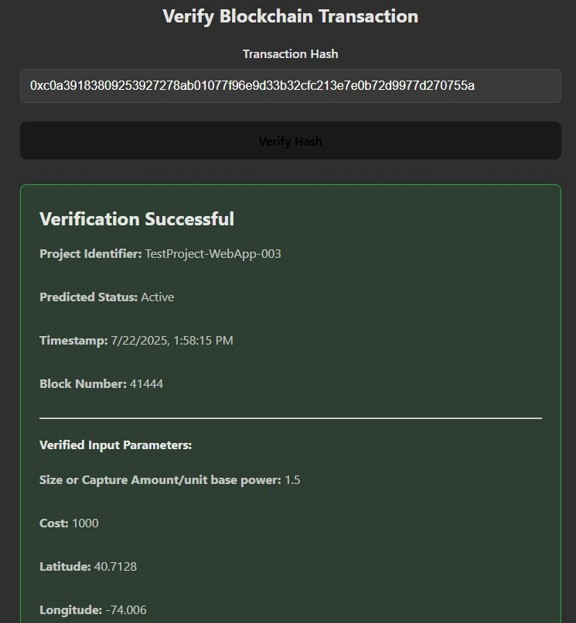
\includegraphics[width=0.48\textwidth]{images/BC Auditability2.jpg}}
\vspace{-0.25cm}
\caption{Purechain blockchain verification interface showing low-latency, zero-cost communication of CCS prediction records}
\label{verify-audit}
\end{figure}



\begin{table*}[htbp]
\scriptsize
\caption{comparative analysis of ai/blockchain frameworks for ccs and carbon management}
\label{framework_comparison}
\centering
\resizebox{\textwidth}{!}{
\begin{tabular}{p{2cm} p{2cm} p{2cm} p{2cm} p{2cm} p{2cm} p{2.2cm}}
\hline \toprule
\textbf{Aspect} &~\cite{abdi2021modeling} & \textbf~\cite{mohammadi2024predictive} &  \textbf{~\cite{aliyon2023use}} & \textbf{~\cite{patro2024blockchain}} & \textbf{~\cite{gupta2025ai}} & \textbf{This Work (Enhanced AI-BC)} \\ \hline
\textbf{Primary Objective} &CO$_2$ adsorption on MOFs & CO$_2$ solubility prediction & Energy cost optimization & Supply chain traceability & Carbon credit verification & \textbf{CCS project status monitoring} \\ 
\textbf{Technology Stack} & XGBoost, CatBoost, LightGBM & XGBoost, CatBoost, LightGBM & AI (Deep Learning) + xAI & Blockchain + IoT + AI & AI + Blockchain + Satellite & \textbf{Ensemble xAI + Purechain BC} \\ 
\textbf{Learning Task} & Regression & Regression& Regression (Reboiler duty) & Conceptual Framework & Validation/Generation & \textbf{Multi-class Classification} \\ 
\textbf{Explainability} & Not addressed& Not addressed& Supported (SHAP) & Not addressed & Not available (Black-box) & \textbf{Integrated Ensemble xAI} \\ 
\textbf{Data Source} & MOFs curated dataset & Experimental data points& ACC Plant simulation & Supply chain metadata & Satellite and IoT sensors & \textbf{Global CCS Project Repository} \\ 
\textbf{Dataset scale}  & 1,191 experimental points &  $>$1,000 lab measurements  & Not available & Not available & Not available & Multi-source CCS project data \\
\textbf{Verification Mode} & Manual assessment& Manual assessment & Manual assessment & Conceptual Ledger & Smart contracts (Conceptual) & \textbf{On-chain Immutable Logging} \\ 
\textbf{Consensus Mechanism} & Not available& Not available& Not available & Not specified & Not specified & \textbf{Low-latency PoA$^{2}$} \\ 
\textbf{Latency/Cost} & Not available & Not available & Not available& Not reported & Not available & \textbf{0.81s / Zero Transaction Cost} \\ 
Result traceability & Not supported & Not supported & Not supported & Not supported & Not supported & On-chain immutable logging \\
Model output auditability & Not available & Not available & Not available & Not available& Not available & Cryptographically verifiable \\
\textbf{System Readiness} & Conceptual& Conceptual & Design-phase assessment & Proof-of-concept vision & Architectural suggestion & \textbf{Deployable ICT Architecture} \\ \hline \toprule
\end{tabular}
}
\end{table*}



\subsection{Performance Evaluation with SOTA CCS Frameworks}
To rigorously evaluate the operational efficacy of the proposed AI-BC architecture, we conducted a comparative performance analysis against contemporary frameworks in the CCS and carbon management domains ~\cite{aliyon2023use}, ~\cite{patro2024blockchain}, ~\cite{gupta2025ai}. While existing studies have pioneered the use of AI for energy cost reduction ~\cite{aliyon2023use} or proposed conceptual blockchain visions for supply chain traceability ~\cite{patro2024blockchain} and carbon credit verification ~\cite{gupta2025ai}, Table~\ref{framework_comparison}  highlights a significant gap in system readiness and empirical validation, which our work proactively addresses.

The significance of our approach is characterized by three primary technical advancements. First, whereas previous works remain largely offline or conceptual ~\cite{abdi2021modeling},
~\cite{mohammadi2024predictive}, ~\cite{patro2024blockchain}, the proposed framework delivers a fully realized, deployable ICT architecture. Empirically, the integration of the Purechain network achieves a sub-second transaction confirmation latency of 0.81 s (with a range of 0.75--0.89 s), a critical metric for real-time industrial CCS monitoring that is conspicuously absent or not reported in competing frameworks. Second, our architecture eliminates the economic barriers to adoption; the utilization of a gasless Purechain infrastructure ensures zero transaction costs, offering a scalable alternative to the high-cost public networks often suggested in broader climate monitoring studies ~\cite{gupta2025ai}. 



Finally, the proposed framework is the first to achieve the ``Technical Trinity" of high predictive accuracy, model-agnostic interpretability, and cryptographic auditability. While Aliyon et al. ~\cite{aliyon2023use} utilize SHAP for energy optimization, their system lacks a secure communication layer to prevent result tampering. Conversely, blockchain-centric models like those by Gupta \& Reddy ~\cite{gupta2025ai} often operate as ``black-boxes" without explainability. By immutably recording both ensemble-based predictions (82\% accuracy) and their associated SHAP-based rationales via a low-latency PoA$^{2}$ consensus mechanism, our framework establishes a new benchmark for trustworthy AI-driven environmental governance. The 100\% verification success rate observed in our experiments confirms that the analytical outputs remain verifiable and traceable throughout the system lifecycle, providing the transparency required for regulatory oversight and operational risk management in next-generation CCS infrastructures.







\vspace{-0.1cm}
\section{\textbf{conclusion and future work}}
\label{con}

This study proposed an ensemble explainable AI--Blockchain framework for predictive and auditable Carbon Capture and Storage (CCS) monitoring, with particular emphasis on ICT-oriented integration and practical deployment. The framework combines stacked ensemble learning using CatBoost, XGBoost, and LightGBM with domain-aware feature interaction design, class-weighted optimization, and SHAP-based explainability to support transparent and reliable multi-class prediction of CCS project status. In addition, the integration of the Purechain permissioned blockchain provides immutable and verifiable logging of model outputs through a low-latency Proof-of-Authority-and-Association consensus mechanism, thereby strengthening trust, traceability, and accountability across distributed CCS stakeholders. The full pipeline, including data preprocessing, ensemble training, interpretability analysis, blockchain interaction, and web-based presentation, was implemented with reproducible software components and evaluated on a real-world global CCS dataset.

Experimental results confirm the effectiveness of the proposed framework. The enhanced ensemble model achieved an overall accuracy of approximately 0.82, a weighted F1-score of about 0.80, and a macro-average performance of 0.68, while one-vs-rest ROC analysis yielded an AUC of approximately 0.87, indicating strong discriminative capability across CCS project classes. The results further showed improved probability calibration and stronger predictive robustness for the dominant \textit{Active} and \textit{Completed} classes, while feature-importance analysis revealed that normalized CO$_2$ capture scale, project cost, and interaction-based variables were among the most influential predictors. On the blockchain side, the Purechain layer achieved sub-second transaction confirmation with an average latency of 0.81 s, zero (0) transaction cost, and a 100\% verification success rate, demonstrating the feasibility of secure and auditable near-real-time CCS prediction logging. Together, these findings show that the framework is capable of delivering accurate, interpretable, and trustworthy support for CCS monitoring and decision-making. 

Despite these contributions, the present evaluation remains limited to static historical CCS records and does not yet include live IoT-enabled sensing streams or continuous model retraining under evolving field conditions. As a result, the adaptability of the framework to rapidly changing operational environments has not yet been fully validated. Future work will therefore focus on extending the system toward real-time data ingestion from distributed monitoring infrastructures, integrating online learning and adaptive model updating under concept drift, and further refining class definitions for transitional project states to improve class separability and operational reliability in large-scale CCS applications.


\vspace{-0.2cm}
\section *{acknowledgment} 
%\scriptsize
\vspace{-0.15cm}
This work was partly supported by Innovative Human Resource Development for Local Intellectualization program through the IITP grant funded by the Korea government (MSIT) (IITP-2026-RS-2020-II201612, 33\%) and by Priority Research Centers Program through the NRF funded by the MEST (2018R1A6A1A03024003, 33\%) and by the MSIT, Korea, under the ITRC support program (IITP-2026-RS-2024-00438430, 34\%).
\balance
\vspace{-0.2cm}
\bibliographystyle{IEEEtran}
\bibliography{newref,Bibliography}

\end{document}

